\section{Mechanical Design and Fabrication}
\label{sec:mech}

The proposal specified a trimaran: a displacement main hull with two
outrigger floats (amas), a self-trimming wingsail, a bulbed fin keel, and a
spade rudder. The as-built ALAN is a monohull. On-water testing showed that
the monohull, with its ballasted fin keel providing the righting moment, was
stable enough for the calm reservoir conditions it was tested in, so the amas
were not included (Section~\ref{sec:integration}). The displacement hull was
chosen for stability, the self-trimming wingsail for its low actuation power,
the fin keel for manufacturability (hull and keel are built separately and
bolted together), the bulb for control over mass and center of gravity, and
the spade rudder because it is the easiest to modify and repair.
Fig.~\ref{fig:cad} shows the complete CAD model.
Table~\ref{tab:changes} summarizes where the as-built vessel departs from the
proposal; the reasons are given in the subsections below.

\begin{figure*}[!t]
\centering
\subfloat[]{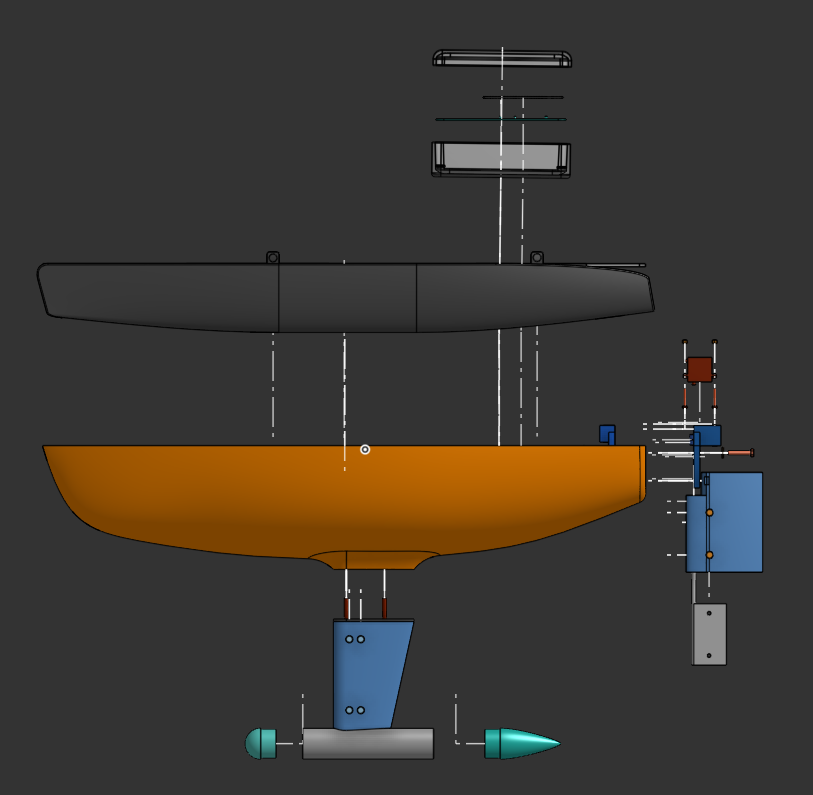
\includegraphics[height=5.2cm]{cad_side}}
\hfil
\subfloat[]{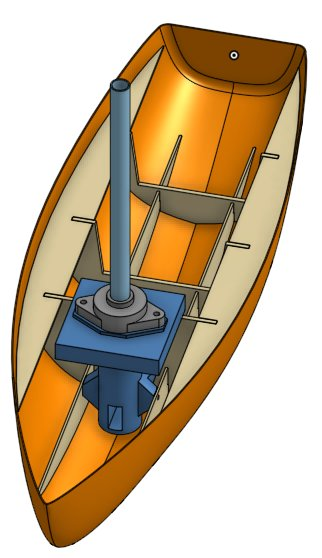
\includegraphics[height=5.2cm]{cad_interior}}
\caption{CAD model. (a) Exploded side view showing the hatch covers, deck, hull,
keel and bulb, and rudder assembly. (b) Hull interior with bulkheads and
the mast step.}
\label{fig:cad}
\end{figure*}

\begin{table*}[!t]
\caption{Changes from the ECE 3992 Proposal}
\label{tab:changes}
\centering
\begin{tabular}{@{}p{0.15\textwidth}p{0.33\textwidth}p{0.45\textwidth}@{}}
\toprule
Item & Proposed & As built \\
\midrule
Tail drive & Servo inside the wing, wire linkage to the tail & Servo at the tail's lower pivot, driving it directly; no linkage backlash \\
Wing skin & Fiberglass over carved XPS foam & Bare carved XPS foam; fiberglass skin planned for the final iteration \\
Mast & Hollow carbon fiber rod & \SI{3}{ft} 6061 aluminum tube in a flanged ball-bearing unit \\
Wing travel & Free rotation & Printed hard stops at $\pm\SI{90}{\degree}$ \\
Sail angle sensing & Estimated from servo position and IMU yaw & AS5600 magnetic encoder at the mast step \\
Ballast & Bulb tube filled with up to \SI{2}{\kilo\gram} of steel balls & Two removable threaded ballast canisters, adjustable at the dock \\
Keel finish & Carbon fiber or fiberglass wrap & Bare printed fairing \\
Electronics housing & Pelican M60 case & Printed enclosure in a sealed deck hatch with cable glands \\
Battery & 3S \SI{11.1}{\volt} LiPo with a battery management system (BMS) & 4S \SI{14.8}{\volt} LiPo with a BMS and per-cell voltage telemetry \\
Orientation & Complementary filter with GPS/IMU dead reckoning & BNO055 onboard nine-axis fusion, quaternion averaging, GPS surge speed \\
Failsafe & Return to home on link loss & SAFE mode and arbiter timeouts; link-loss timeout implemented but not yet enabled \\
Hull form & Trimaran (main hull with two amas) & Monohull; ballasted keel provides the righting moment \\
\bottomrule
\end{tabular}
\end{table*}

\subsection{Hull}
The hull is a wet layup of fiberglass and epoxy in a two-piece female mold.
The mold was 3D printed in polylactic acid (PLA) in bow and stern halves that bolt together
(Fig.~\ref{fig:hull}(a)), then surfaced with filler primer and a 2K gloss
topcoat, waxed, and coated with a polyvinyl alcohol (PVA) film release agent. Seven plies of \SI{4}{oz} plain-weave fiberglass
laid up with 5:1 marine epoxy give a cured wall thickness of about
\SI{1}{\milli\meter}. The keel mount was
reinforced with additional plies and a metal plate laminated inside the mount
boss; the transom received extra plies but a removable internal plate, so
that rudder hardware can be serviced. Bulkheads and the sail templates were
laser cut from plywood (Fig.~\ref{fig:hull}(b)) and bonded into the hull to
stiffen it and to locate the mast step.

The deck is extruded polystyrene (XPS) foam board laminated with fiberglass
and resin. Two printed hatch coamings are bonded into the deck, and each
hatch cover is held by four printed over-center latches
(Fig.~\ref{fig:deck}(a)). Cable penetrations use compression cable glands.

\begin{figure}[!t]
\centering
\subfloat[]{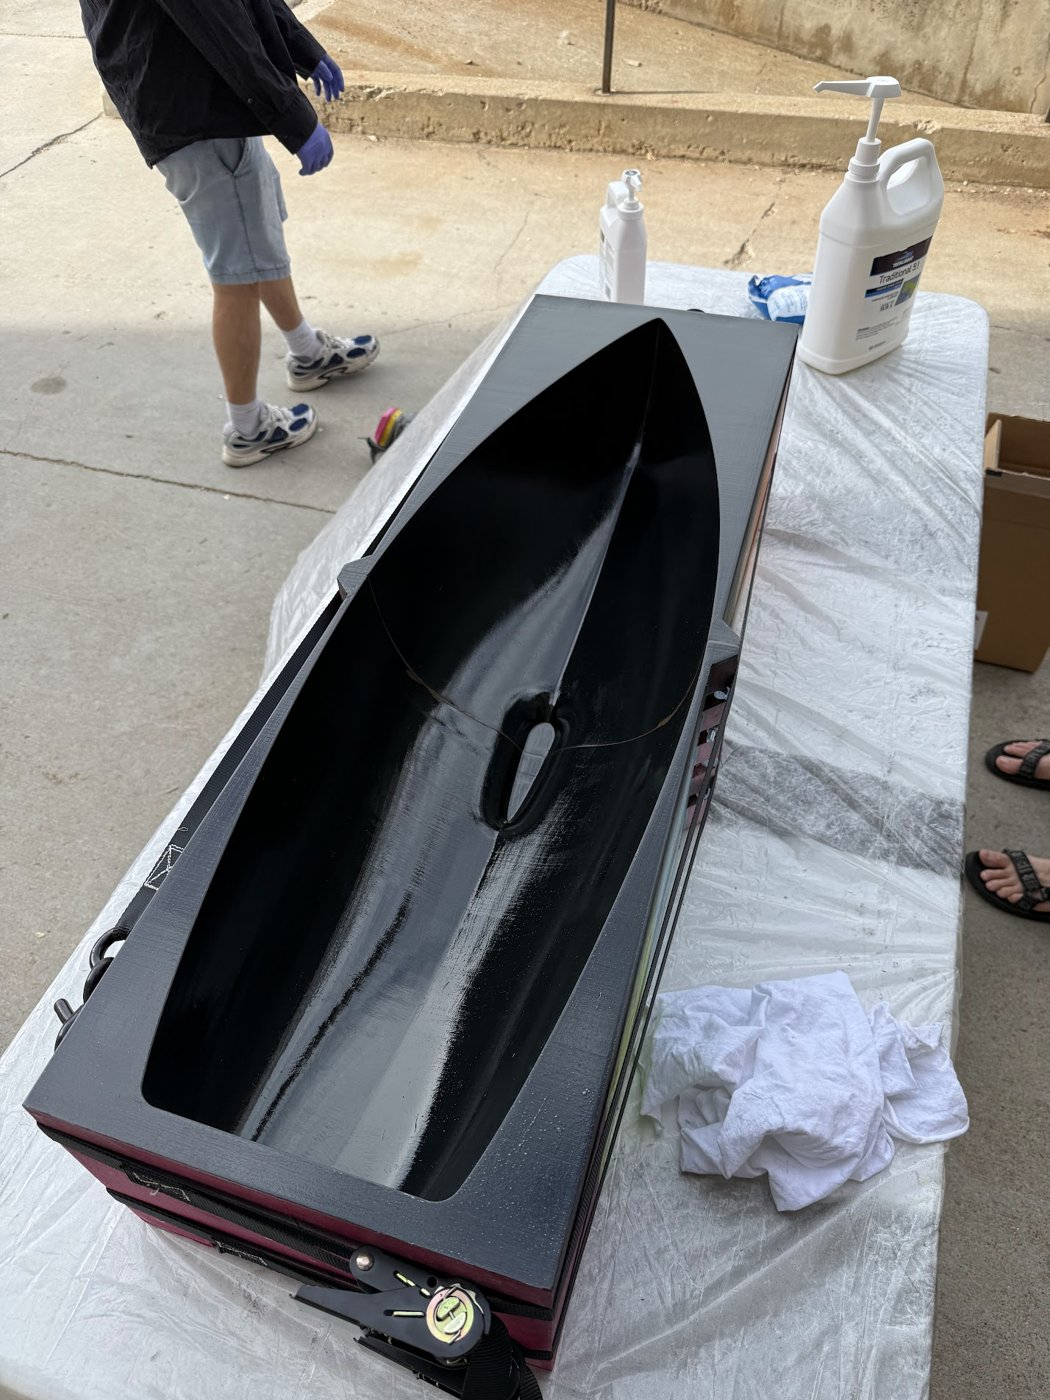
\includegraphics[height=4.4cm]{hull_mold}}
\hfil
\subfloat[]{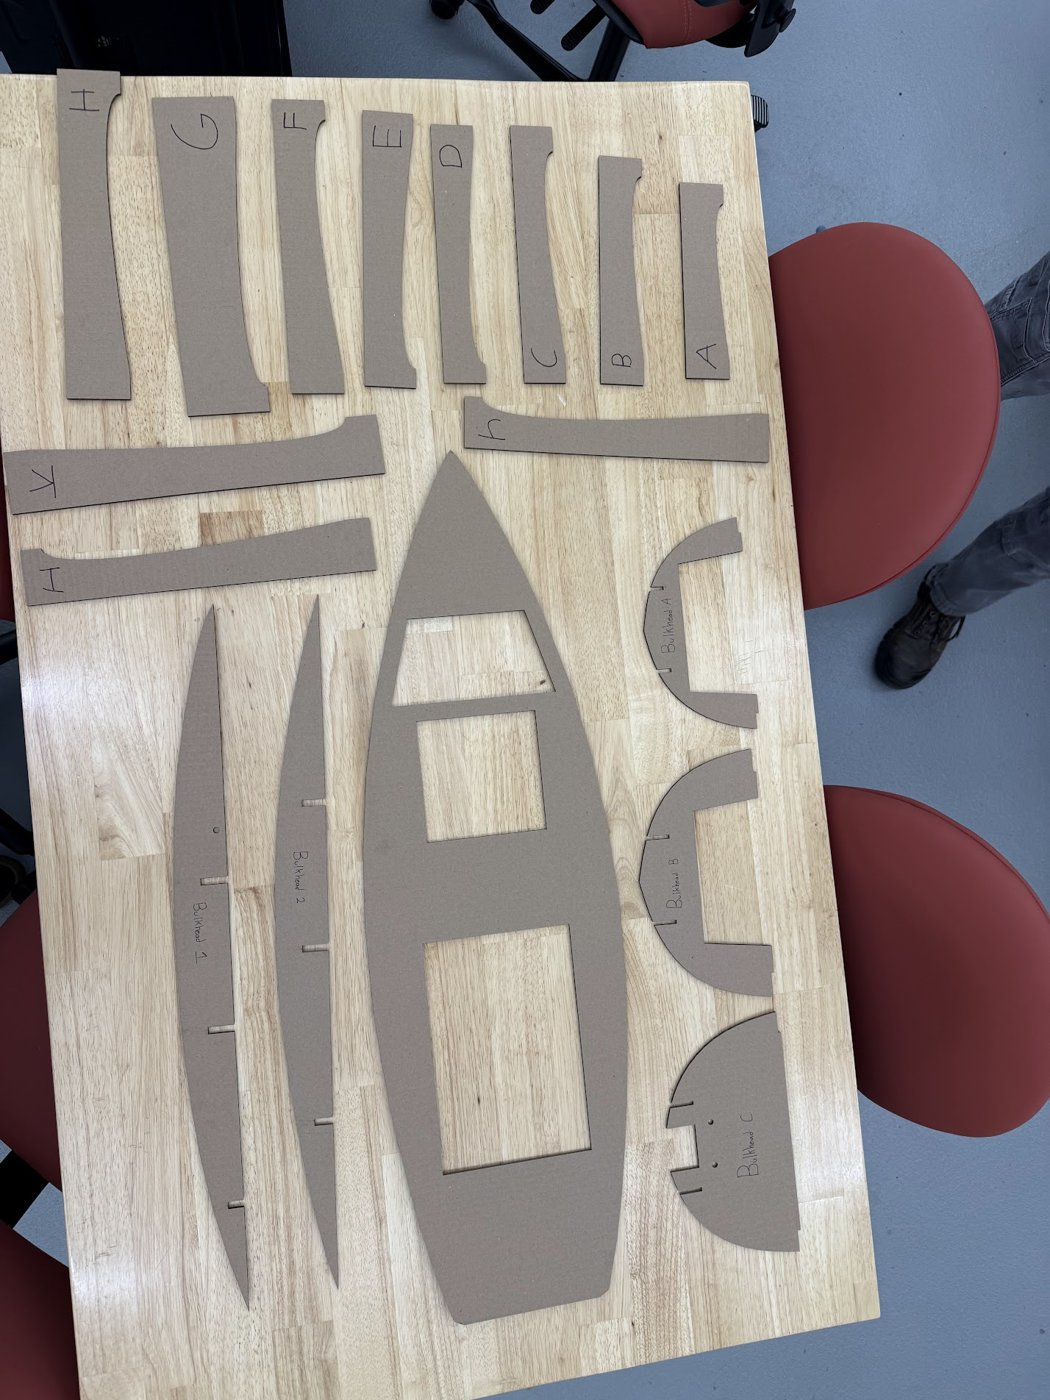
\includegraphics[height=4.4cm]{laser_cut}}
\caption{Hull fabrication. (a) Printed two-piece female mold prepared for the
fiberglass layup. (b) Laser-cut plywood bulkheads and sail templates.}
\label{fig:hull}
\end{figure}

\begin{figure}[!t]
\centering
\subfloat[]{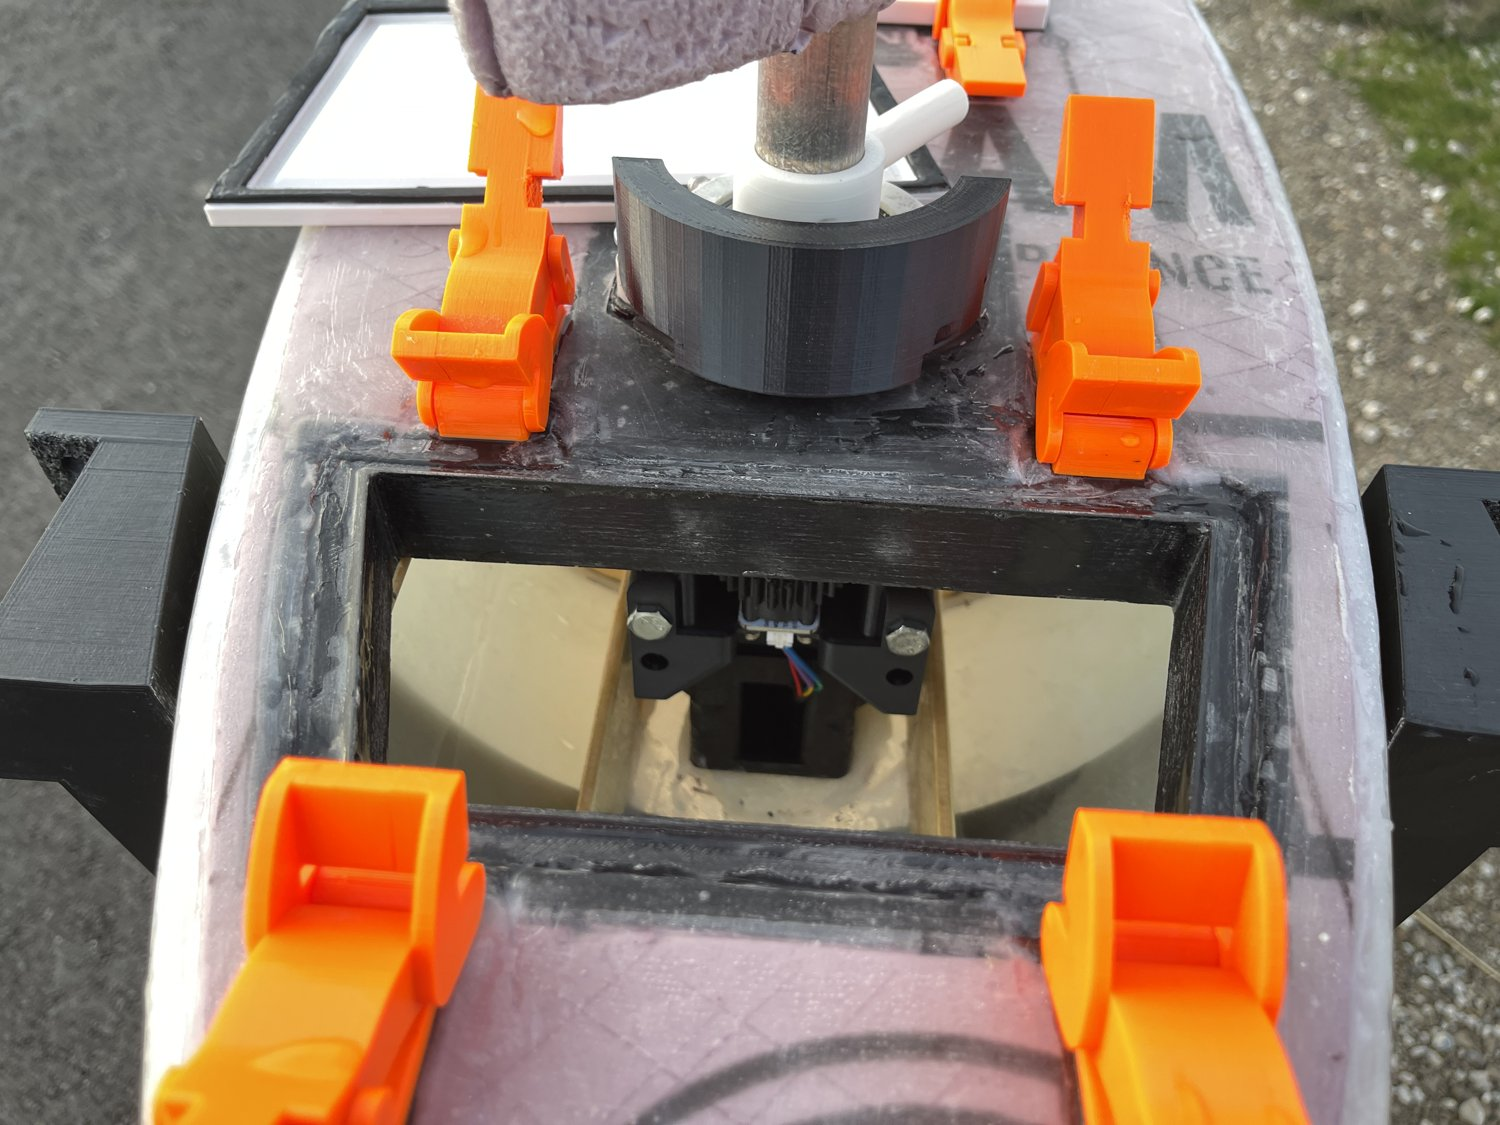
\includegraphics[height=3.9cm]{bow_deck}}
\hfil
\subfloat[]{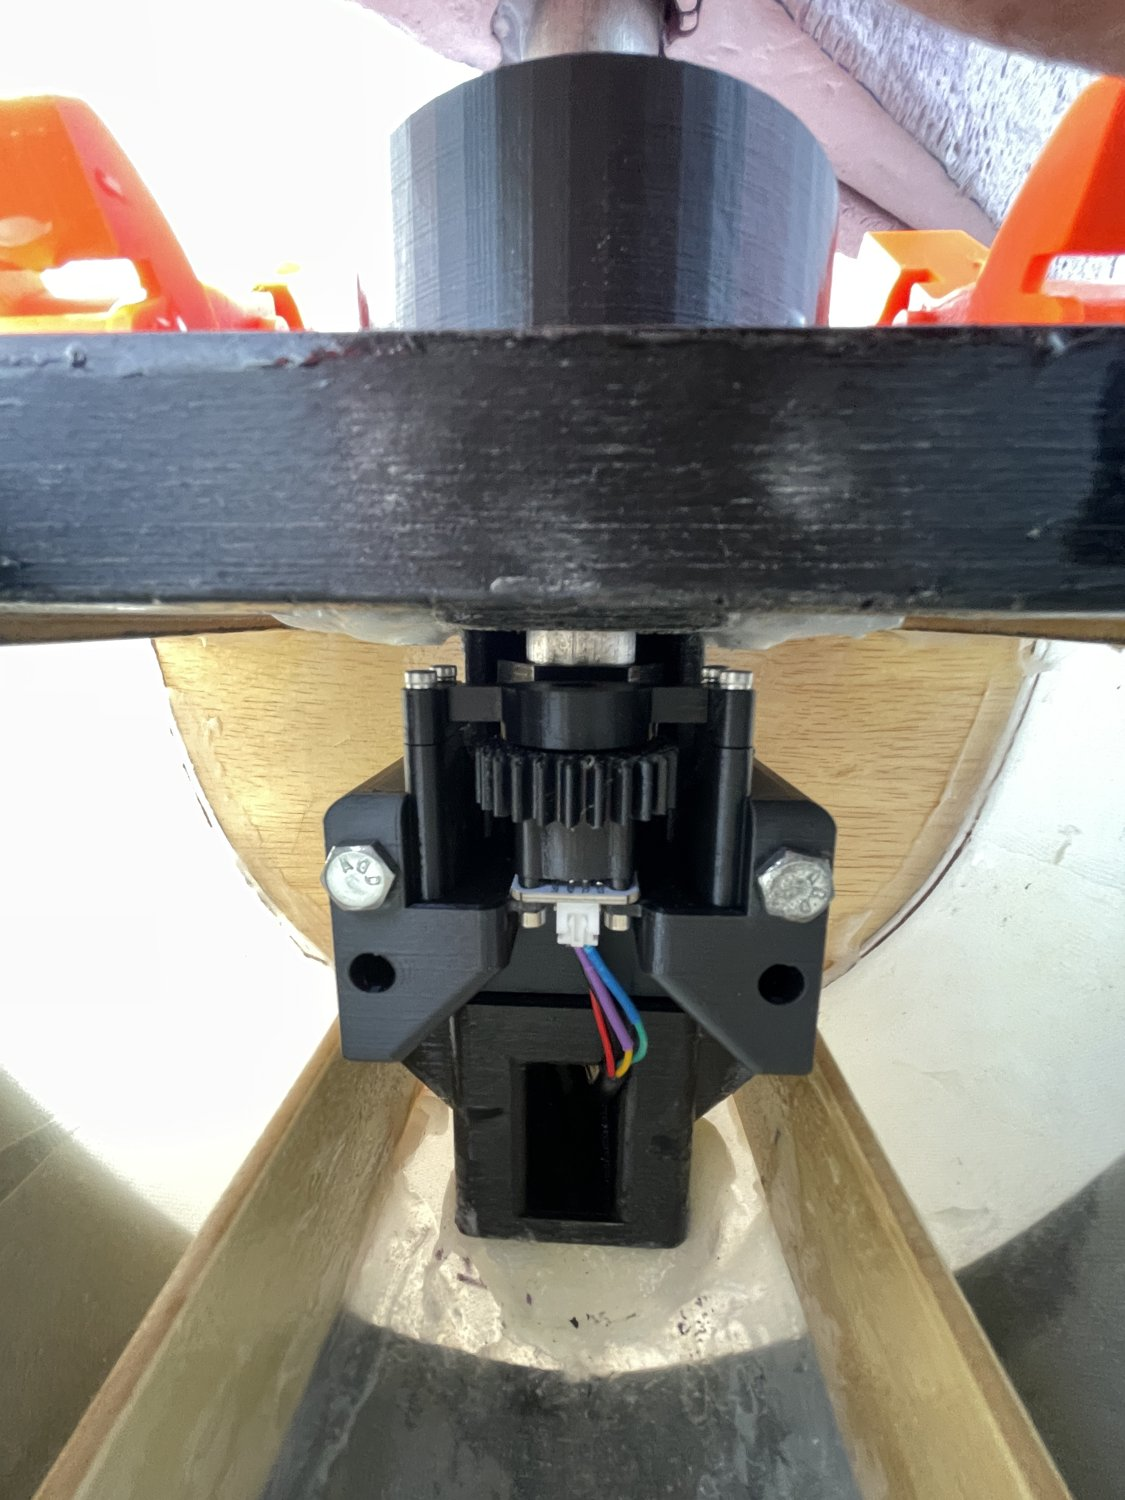
\includegraphics[height=3.9cm]{mast_encoder}}
\caption{Forward deck. (a) Mast base with its collar and guard ring, the
forward hatch open with the encoder assembly visible below, and the printed
over-center latches. (b) Below deck: spur gear and AS5600 magnetic encoder that measure the wing angle
relative to the hull.}
\label{fig:deck}
\end{figure}

\subsection{Keel and Ballast Bulb}
The keel has three parts: a frame, a fairing, and ballast
(Fig.~\ref{fig:keel}). The frame is 304 stainless steel, chosen for its
corrosion resistance: a \SI{0.25}{in} plate mounting bracket, a
\SI{0.5}{in} $\times$ \SI{7}{in} square-bar post, and a \SI{2}{in}
$\times$ \SI{8.5}{in} round tube that forms the core of the bulb. The bracket
bolts through the reinforced keel boss with 1/4-20 bolts and nylon-insert
lock nuts. Two mirrored printed PLA fairing halves clamp around the post with
four bolts and give the keel its foil
section, sized to place the CLR correctly relative to the sail's
COE~\cite{noahrudder,skene2001}.

The proposal called for filling the bulb tube with steel shot. Instead, the
ballast is carried in two stainless canisters that slide into the bulb tube
from either end and are retained by threaded studs
(Fig.~\ref{fig:keel}(c)). A rounded printed nose cap and a tapered tail cap
fair the ends. Because each canister can be loaded independently, the ballast
mass and its fore-aft position can be changed at the dock to trim the boat
without opening the keel. Rust streaks below the fairing bolts in
Fig.~\ref{fig:keel}(b) come from zinc-plated fasteners; these should be
replaced with stainless hardware before extended use in water.

\begin{figure}[!t]
\centering
\subfloat[]{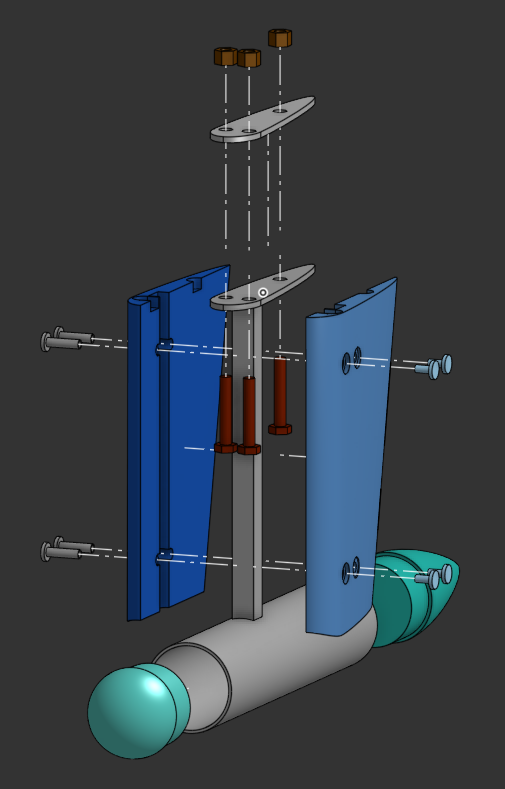
\includegraphics[height=3.0cm]{cad_keel}}
\hfil
\subfloat[]{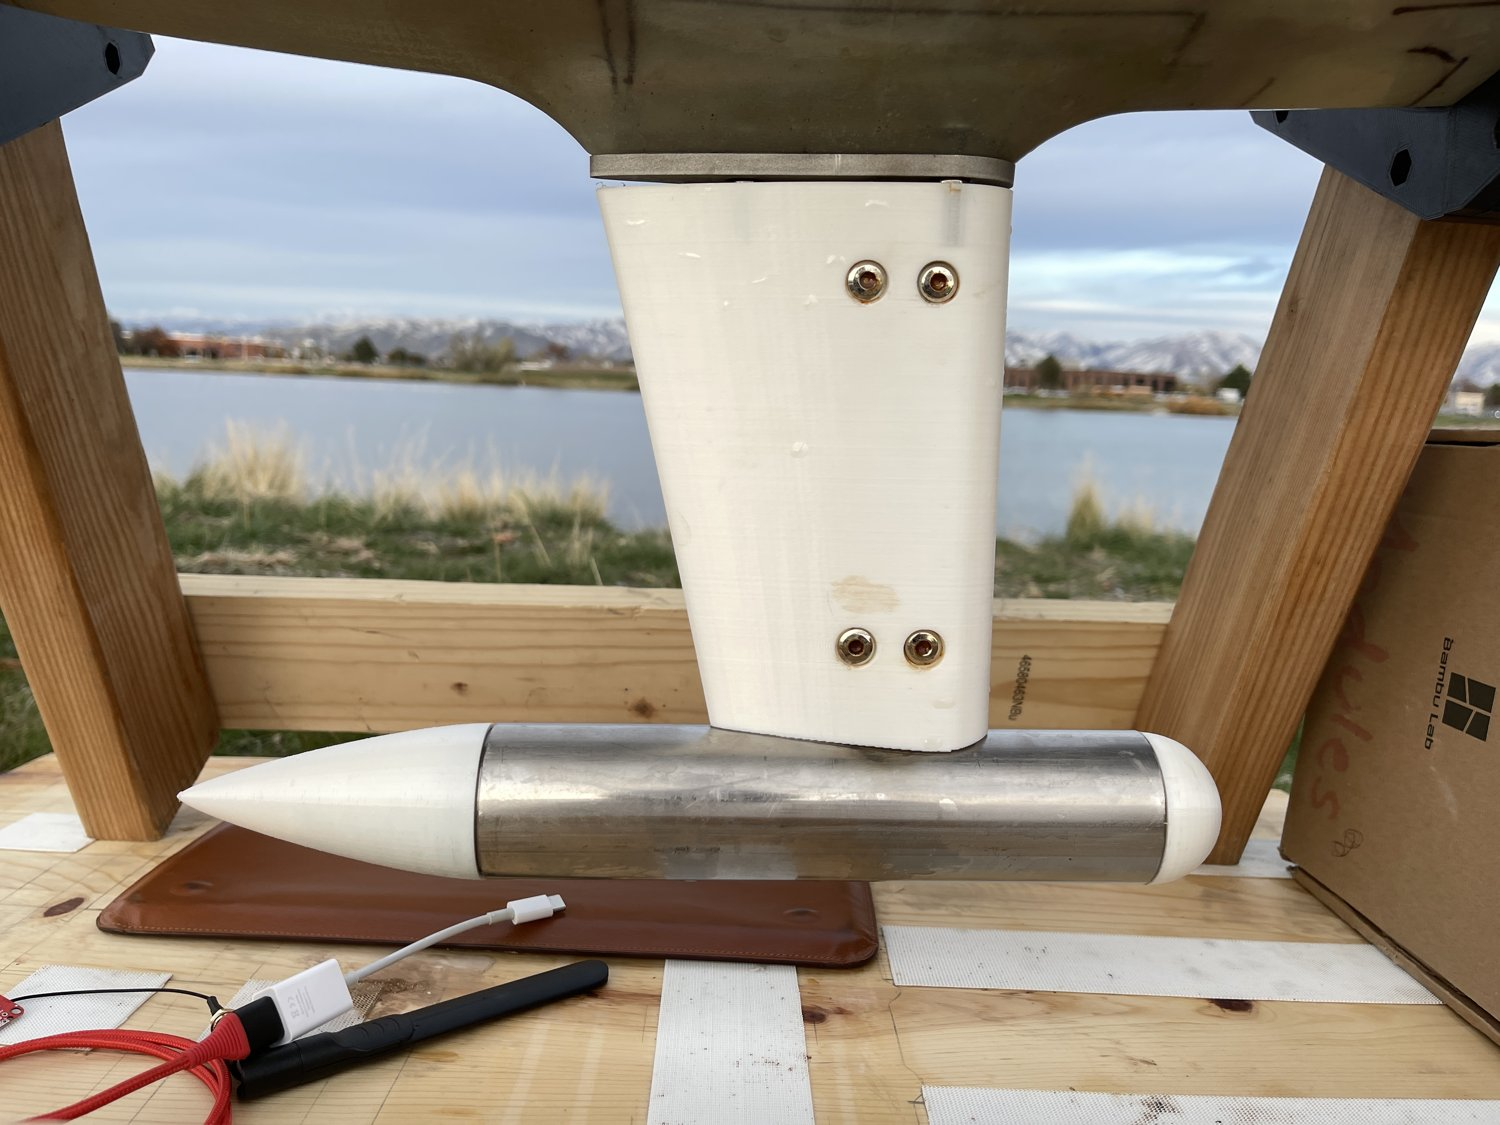
\includegraphics[height=3.0cm]{keel_bulb}}
\hfil
\subfloat[]{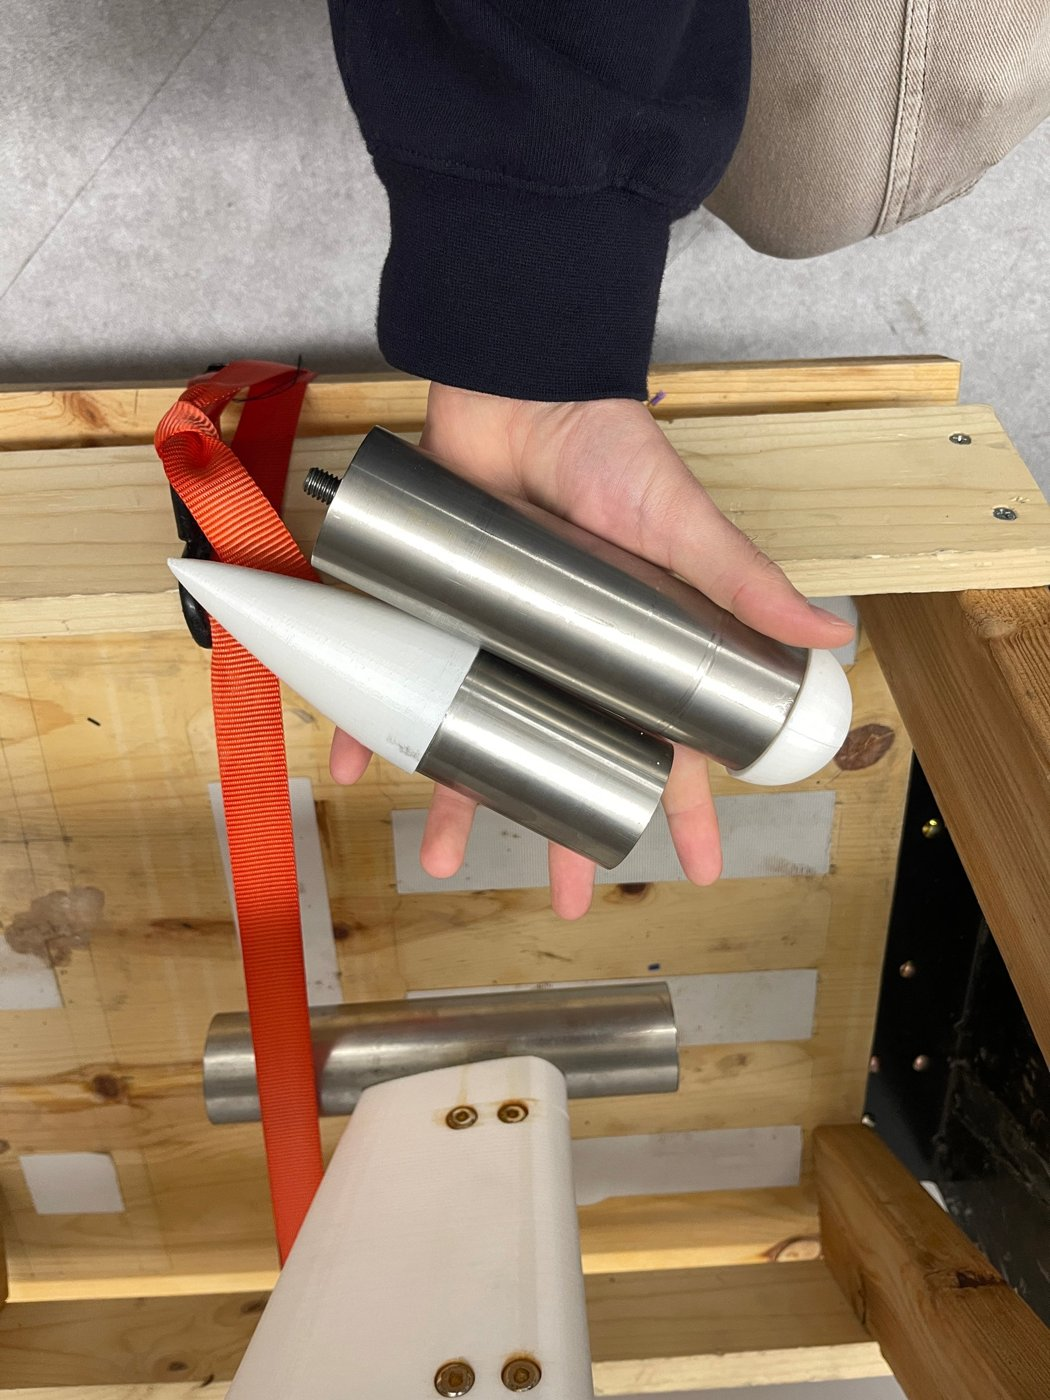
\includegraphics[height=3.0cm]{ballast_canisters}}
\caption{Keel. (a) Exploded CAD of the steel frame, fairing halves, and bulb.
(b) As built, with the fairing bolted to the post and the bulb caps fitted.
(c) Removable ballast canisters with their nose and tail caps.}
\label{fig:keel}
\end{figure}

\subsection{Rudder}
The spade rudder hangs from a \SI{0.25}{in} $\times$ \SI{12}{in} 304
stainless round-bar shaft. A printed rudder blade clamps around the shaft and
is pinned with a cross bolt and barrel nut, so blades of different area can
be swapped without disturbing the shaft. The shaft turns in two R188 ceramic
ball bearings, chosen for corrosion resistance, held in a two-part clamp. The
fore section of the clamp sits against the inside of the transom and the aft
section, with \SI{0.065}{in} aluminum mounting plates, clamps over it with
1/4-20 bolts and nylon-insert lock nuts, so the assembly can be
removed without cutting the hull (Fig.~\ref{fig:rudder}(a)). A DS3218MG
\SI{20}{kg\cdot cm} waterproof digital servo in a printed transom mount
drives the shaft through a 25-tooth spline to 1/4-in.\ bore coupler
(Fig.~\ref{fig:rudder}(b)); Fig.~\ref{fig:rudder}(c) shows the blade. In the
CAD model the blade has a \SI{70}{\milli\meter} chord and a
\SI{100}{\milli\meter} span, an area of \SI{70}{\centi\meter\squared}.

\begin{figure}[!t]
\centering
\subfloat[]{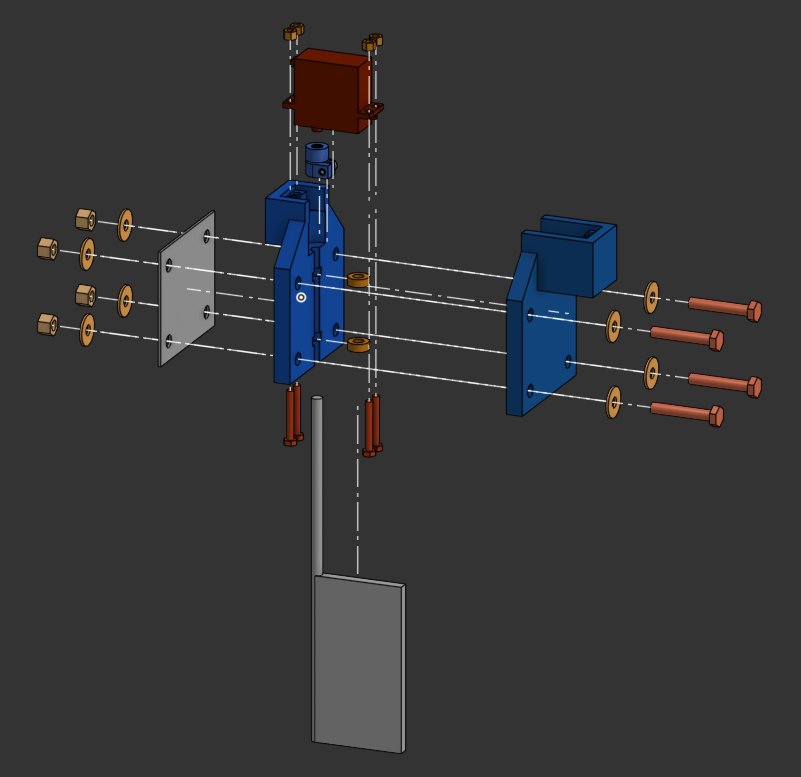
\includegraphics[height=3.2cm]{cad_rudder}}
\hfil
\subfloat[]{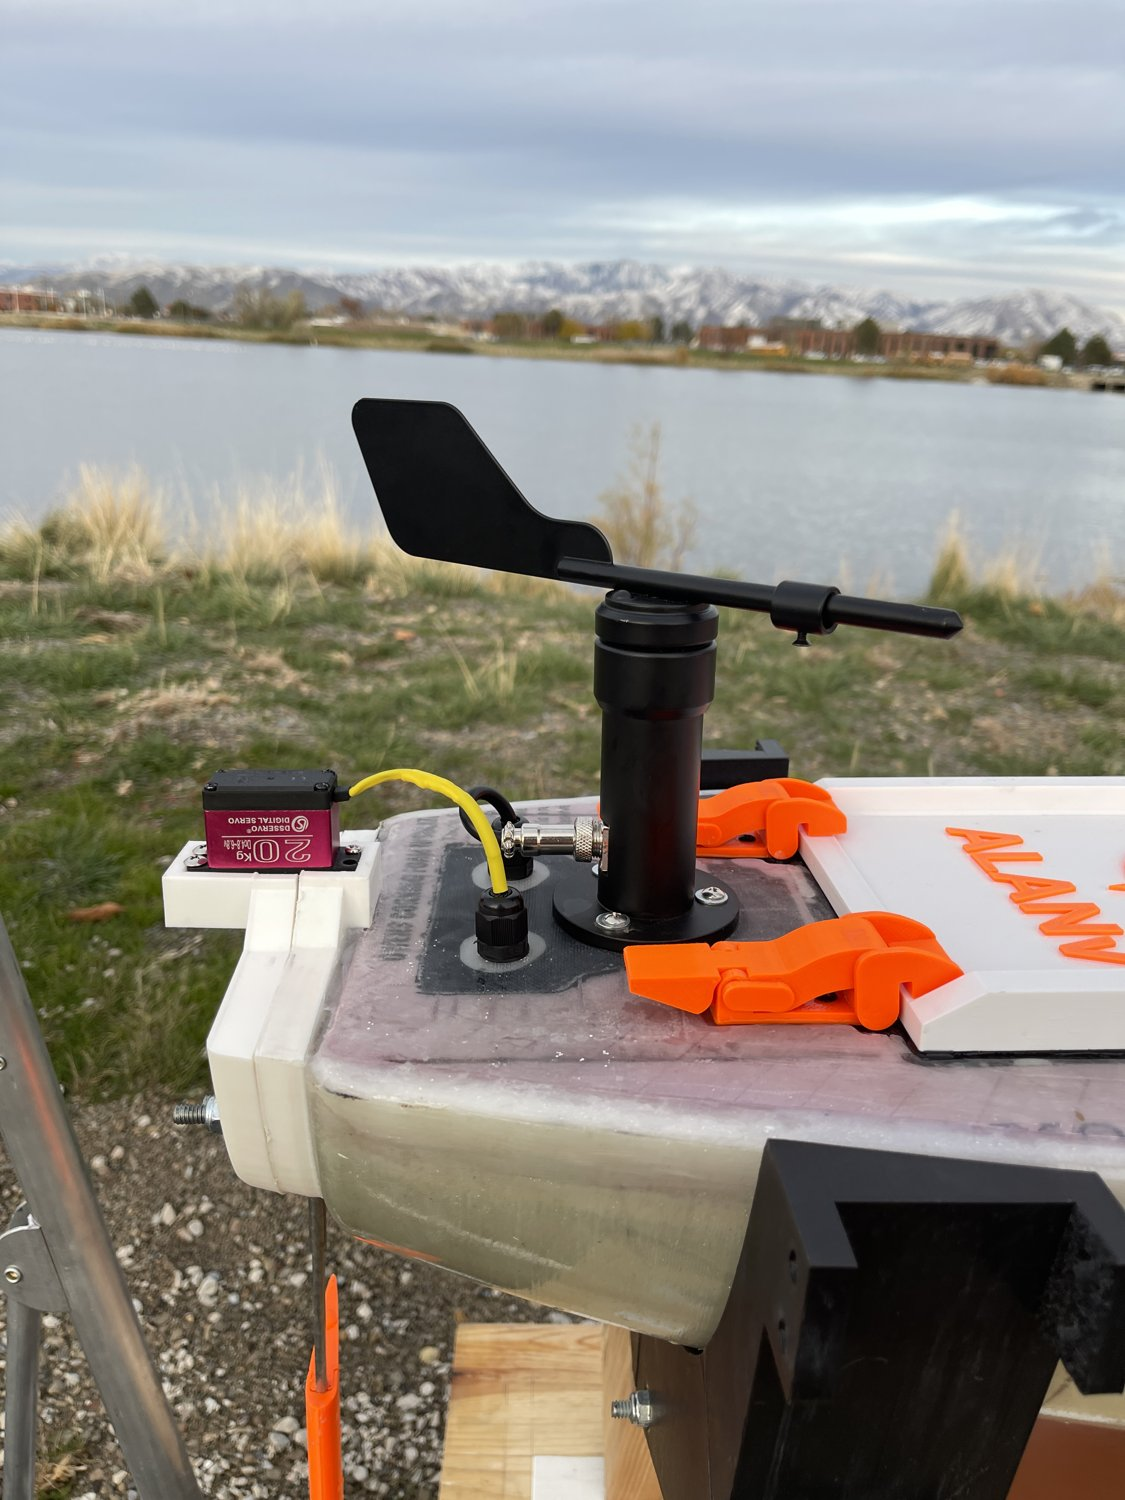
\includegraphics[height=3.2cm]{stern_deck}}
\hfil
\subfloat[]{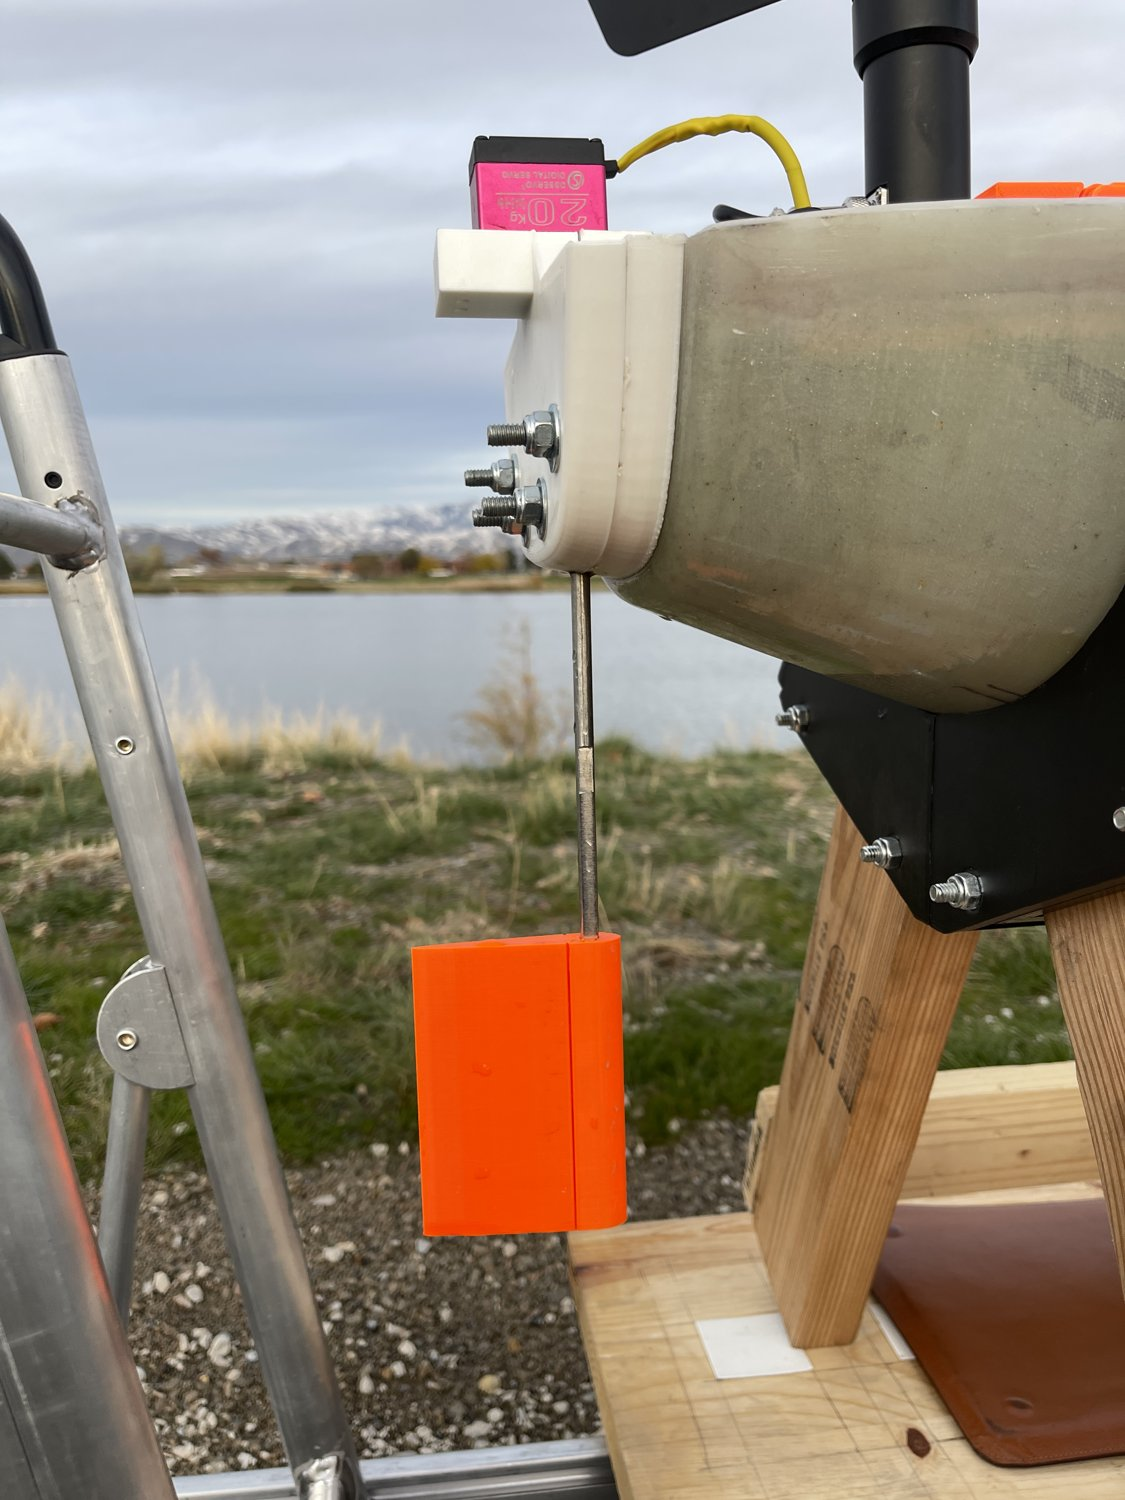
\includegraphics[height=3.2cm]{rudder_photo}}
\caption{Stern. (a) Exploded CAD of the rudder clamp, bearings, and shaft.
(b) Wind vane with its sealed aviation connector, cable glands, and the
rudder servo on its transom mount. (c) Printed rudder blade on the stainless
shaft below the transom.}
\label{fig:rudder}
\end{figure}

\subsection{Self-Trimming Wingsail}
The main wing and tail were carved from laminated XPS foam, which allowed a
wing more than \SI{1}{\meter} tall while keeping its mass low. The wing is
fixed to a \SI{3}{ft} 6061 aluminum mast tube that turns freely in a flanged ball-bearing unit at
deck level (Fig.~\ref{fig:sail}(d)). A printed collar with a radial arm
clamps the mast above the bearing and travels inside a printed guard ring
whose ends are hard stops, limiting the wing to $\pm\SI{90}{\degree}$ from
the centerline. A self-trimming wing never needs to point further aft than
abeam, and the stops protect the tail-servo cable routed through the mast. A \SI{10}{dBi} whip antenna for the
\SI{915}{\mega\hertz} radio is mounted at the masthead on a \SI{5}{ft} SubMiniature version A (SMA)
extension cable, which gives the radio the highest available mounting point
and a clear line of sight (Fig.~\ref{fig:sail}(e)).

Two carbon fiber booms carry the tail aft of the wing. In the proposal, a
servo inside the wing pushed and pulled the tail through a wire. As built,
the servo sits in a printed bracket on the lower boom and turns the tail's
lower pivot directly (Fig.~\ref{fig:sail}(b)), while the upper pivot runs in
a printed bearing housing on the upper boom (Fig.~\ref{fig:sail}(c)). Direct
drive removes the wire's backlash and stretch. The booms extend forward of the
mast to a printed counterweight (Fig.~\ref{fig:sail}(a)) sized so that
\begin{equation}
m_{cw}\, r_{cw} = \sum_i m_i\, r_i ,
\label{eq:balance}
\end{equation}
where the right-hand side sums the mass moments of the tail, servo, and aft
booms about the mast axis. Satisfying \eqref{eq:balance} places the combined center of gravity on the axis, so heel and pitch do not apply a rotating moment to the wing.

\begin{figure}[!t]
\centering
\begin{tikzpicture}[scale=0.95, every node/.style={font=\scriptsize}]
  % apparent wind (from left, +x)
  \foreach \y in {1.3,0.9}
    \draw[-{Latex[length=2mm]},thick,blue!70!black] (-3.6,\y) -- (-2.6,\y);
  \node[blue!70!black,anchor=south] at (-3.1,1.35) {apparent wind};
  \draw[dashed,gray] (-2.4,0) -- (4.4,0);
  \begin{scope}[rotate=-10]
    % boom
    \draw[thick] (-1.7,0) -- (3.6,0);
    % main wing (leading edge at -0.5, pivot at 0)
    \draw[fill=gray!25] (-0.5,0) .. controls (-0.45,0.28) and (0.35,0.3) .. (1.5,0)
                       .. controls (0.35,-0.3) and (-0.45,-0.28) .. (-0.5,0);
    % counterweight
    \fill[gray!60!black] (-1.7,0) circle (0.16);
    \node[anchor=north] at (-1.7,-0.3) {counterweight};
    % tail, deflected by delta about its pivot at 3.2
    \begin{scope}[shift={(3.2,0)}, rotate=22]
      \draw[fill=gray!25] (-0.2,0) .. controls (-0.18,0.12) and (0.15,0.13) .. (0.6,0)
                         .. controls (0.15,-0.13) and (-0.18,-0.12) .. (-0.2,0);
      \draw[densely dotted] (0,0) -- (1.0,0);
    \end{scope}
    \fill[white,draw=black] (3.2,0) circle (0.05);
    \draw[densely dotted] (3.2,0) -- (4.3,0);
    \draw[-{Stealth[length=1.5mm]}] (4.05,0) arc (0:22:0.85);
    \node at (4.25,0.3) {$\delta$};
    \node[anchor=north] at (2.45,-0.22) {tail and servo};
    % mast pivot
    \fill[white,draw=black,thick] (0,0) circle (0.07);
    \node[anchor=north] at (-0.15,-0.32) {mast pivot};
    % lift arrows
    \draw[-{Stealth[length=2mm]},red!70!black,thick] (0.3,0) -- (0.3,1.0) node[above] {$L_w$};
    \draw[-{Stealth[length=2mm]},red!70!black,thick] (3.3,0) -- (3.3,-0.75) node[below left=-2pt] {$L_t$};
  \end{scope}
  % angle of attack
  \draw[-{Stealth[length=1.5mm]}] (1.95,0) arc (0:-10:1.95);
  \node at (2.12,-0.17) {$\alpha$};
\end{tikzpicture}
\caption{Self-trimming wingsail seen from above. Deflecting the tail by
$\delta$ produces a tail lift $L_t$ whose moment about the mast pivot rotates
the wing until it balances the wing lift moment, settling at angle of attack
$\alpha$.}
\label{fig:stw}
\end{figure}

Fig.~\ref{fig:stw} shows why the wing trims itself. With dynamic pressure
$q$, wing and tail areas $S_w$ and $S_t$, signed moment arms $l_w$ and $l_t$
from the pivot to each surface's aerodynamic center, and lift coefficients
$C_{L,w}$ and $C_{L,t}$, the yawing moment about the mast is
\begin{equation}
M(\alpha,\delta) = q \left[ S_w l_w C_{L,w}(\alpha) + S_t l_t C_{L,t}(\alpha-\delta) \right].
\label{eq:moment}
\end{equation}
The wing rotates until $M = 0$ in \eqref{eq:moment}. Because $q$ multiplies both terms, the
equilibrium angle of attack depends on the tail deflection $\delta$ but not on
wind speed~\cite{elkaim2008}. Gusts therefore change the force on the sail but
not its trim, and shifts in wind direction are followed passively. Wind speed
does set how quickly the wing reaches equilibrium, which is the delayed
response noted in Table~\ref{tab:sailtypes} and the main challenge for the
sail controller in Section~\ref{sec:sw}.

\begin{figure*}[!t]
\centering
\subfloat[]{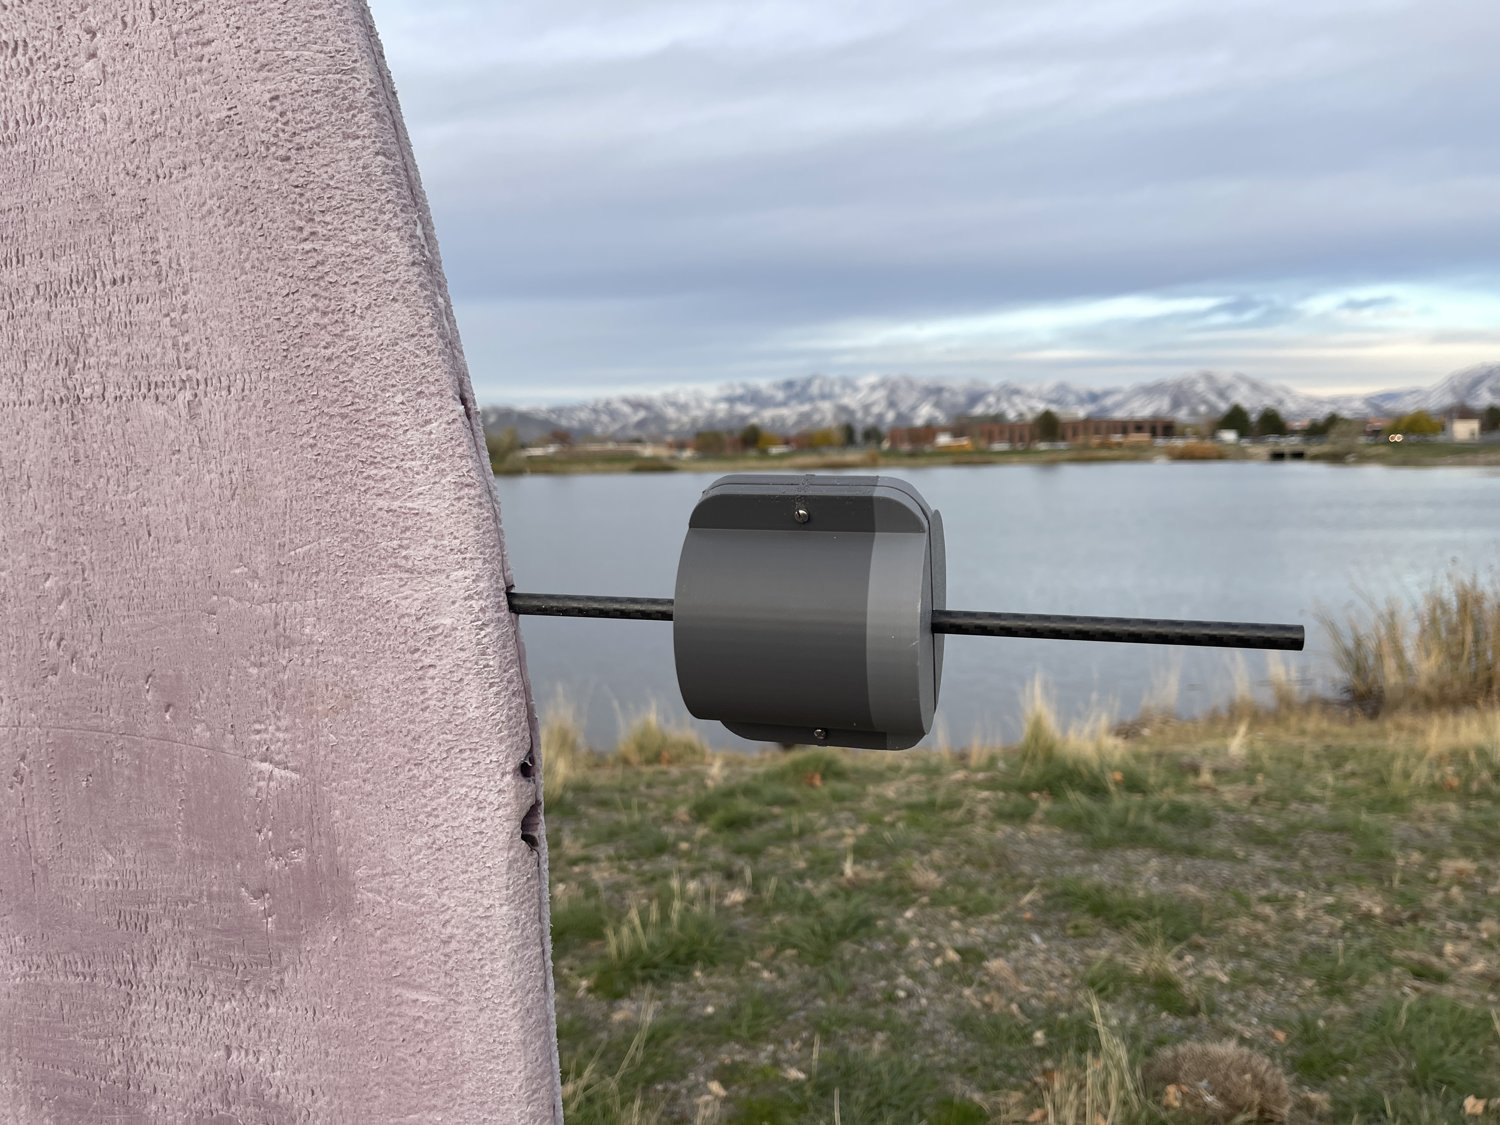
\includegraphics[height=2.55cm]{counterweight}}
\hfil
\subfloat[]{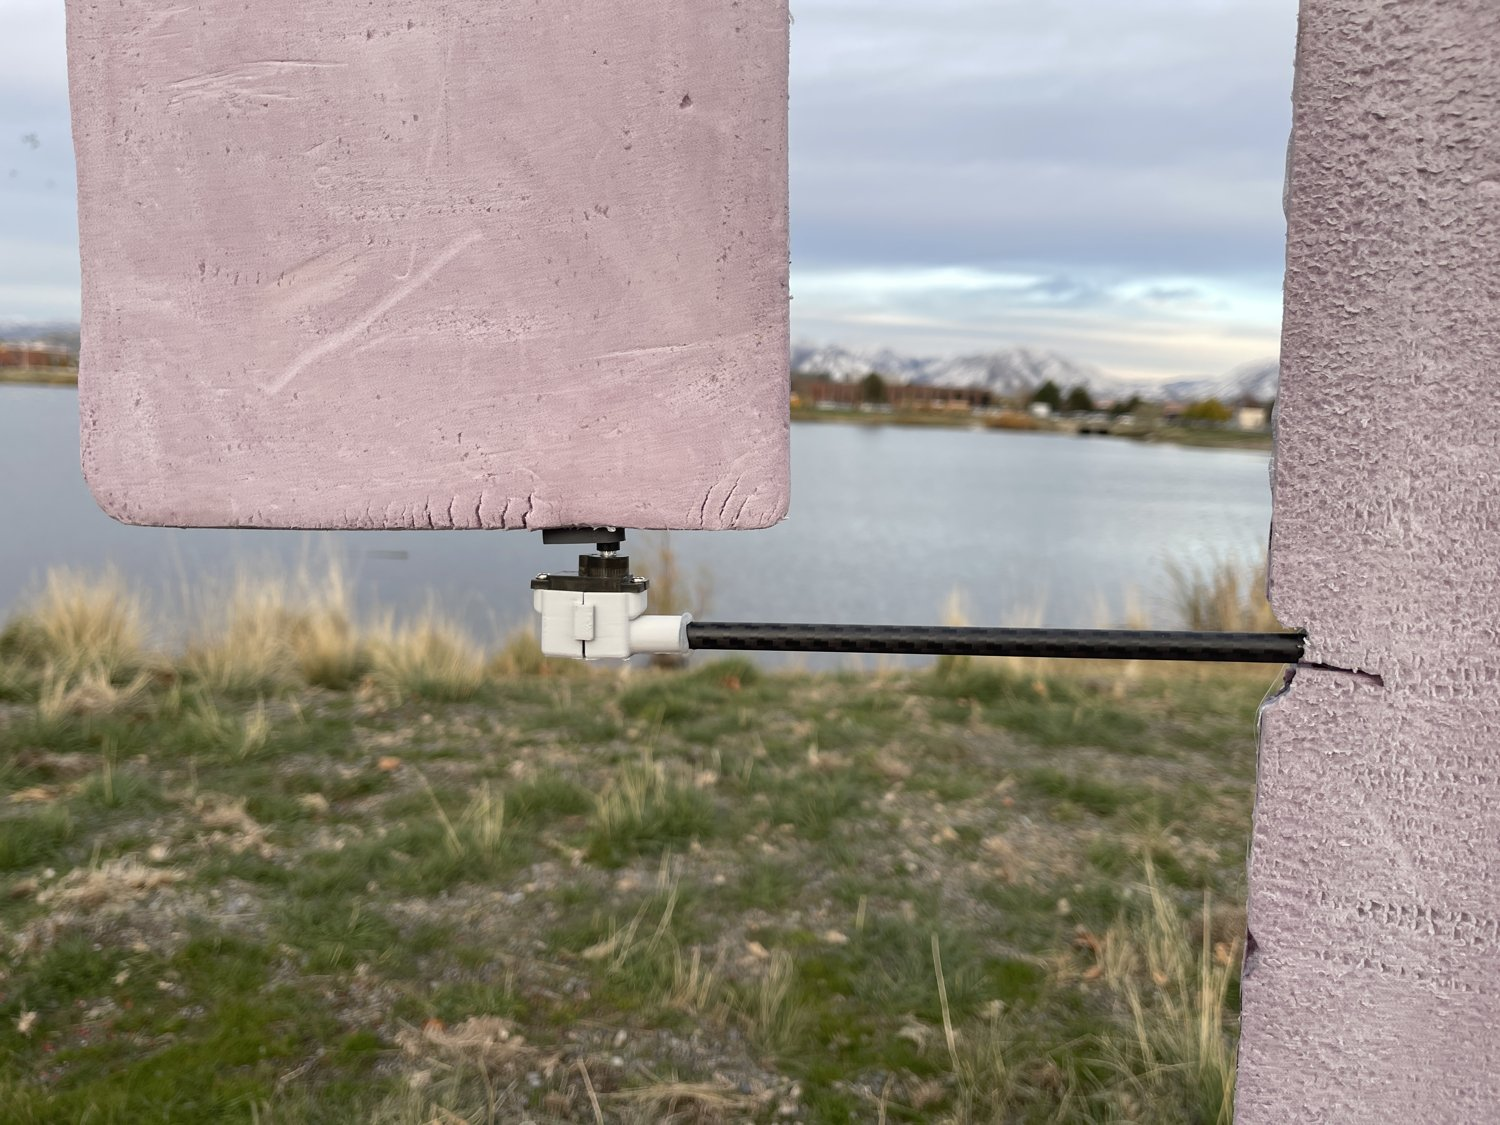
\includegraphics[height=2.55cm]{tail_servo}}
\hfil
\subfloat[]{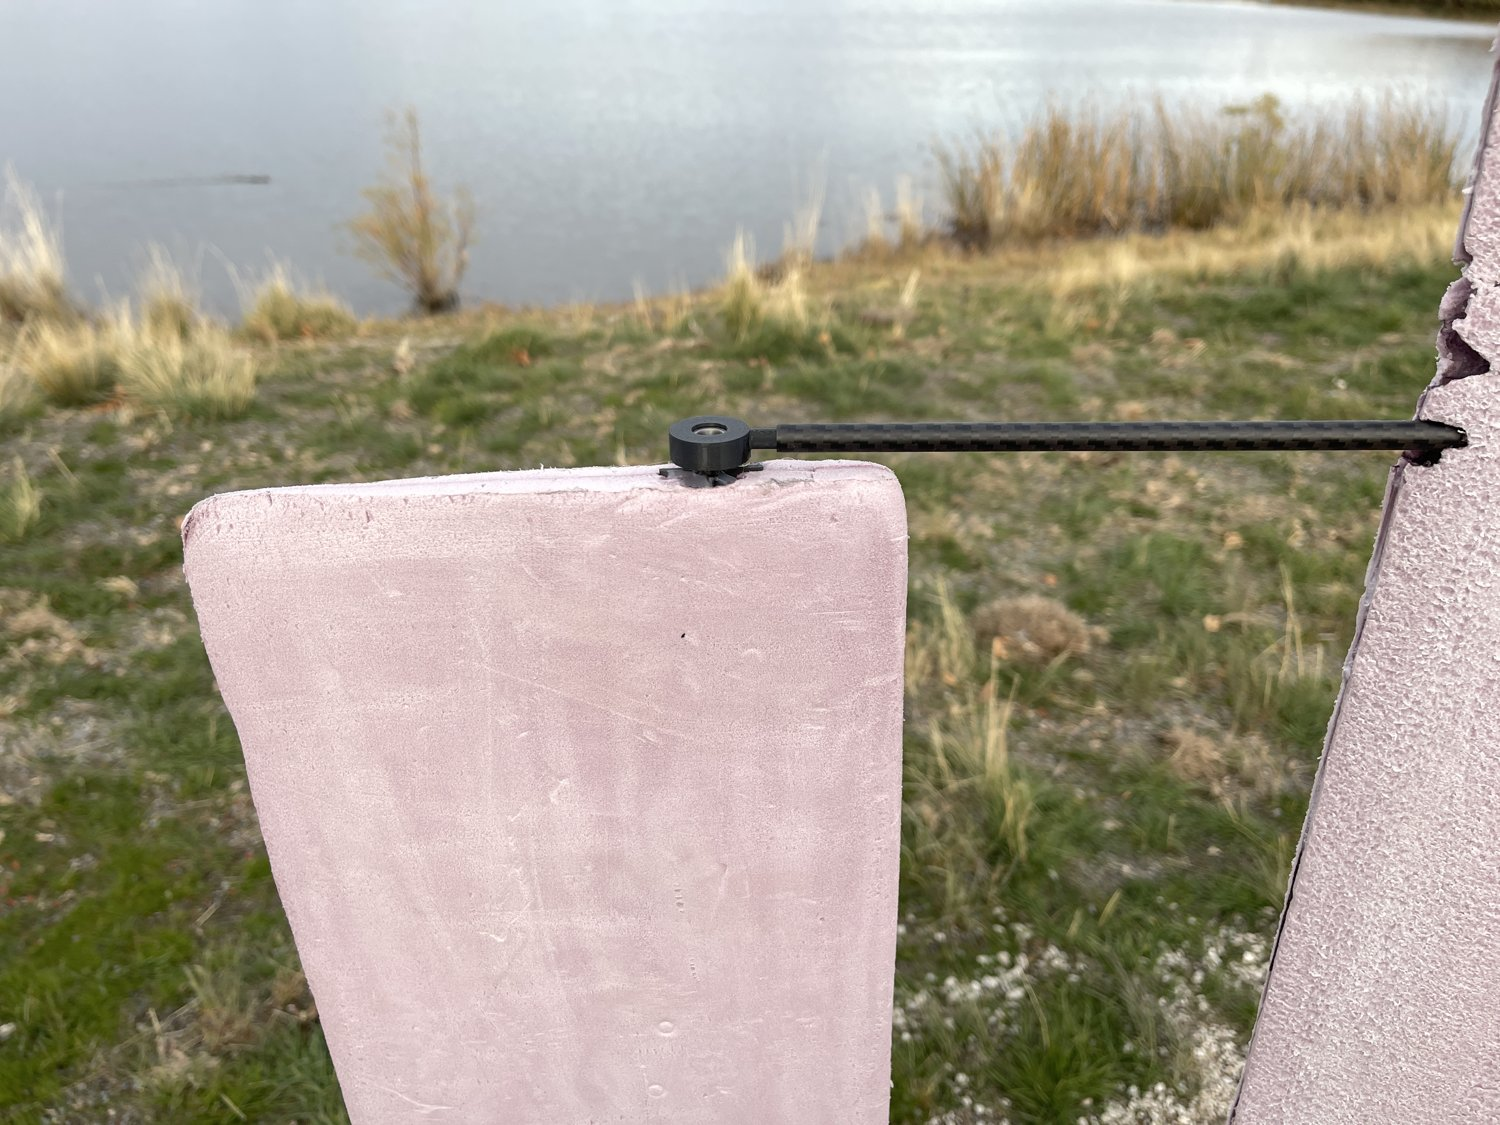
\includegraphics[height=2.55cm]{tail_pivot}}
\hfil
\subfloat[]{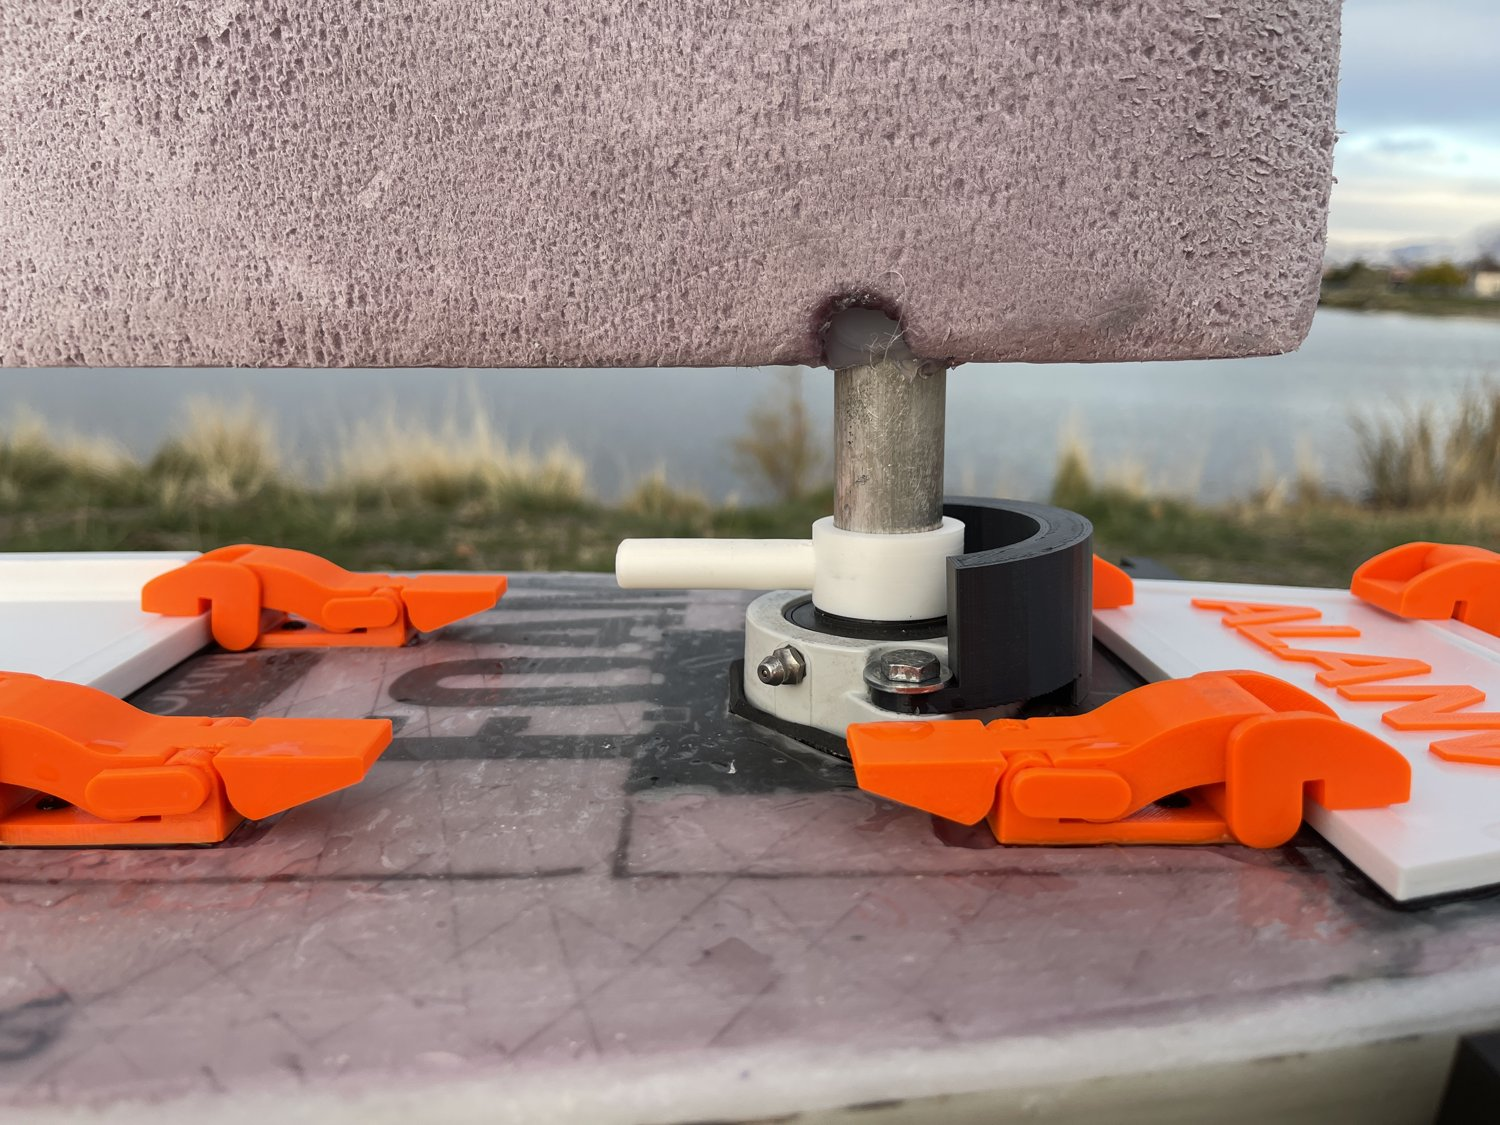
\includegraphics[height=2.55cm]{mast_base}}
\hfil
\subfloat[]{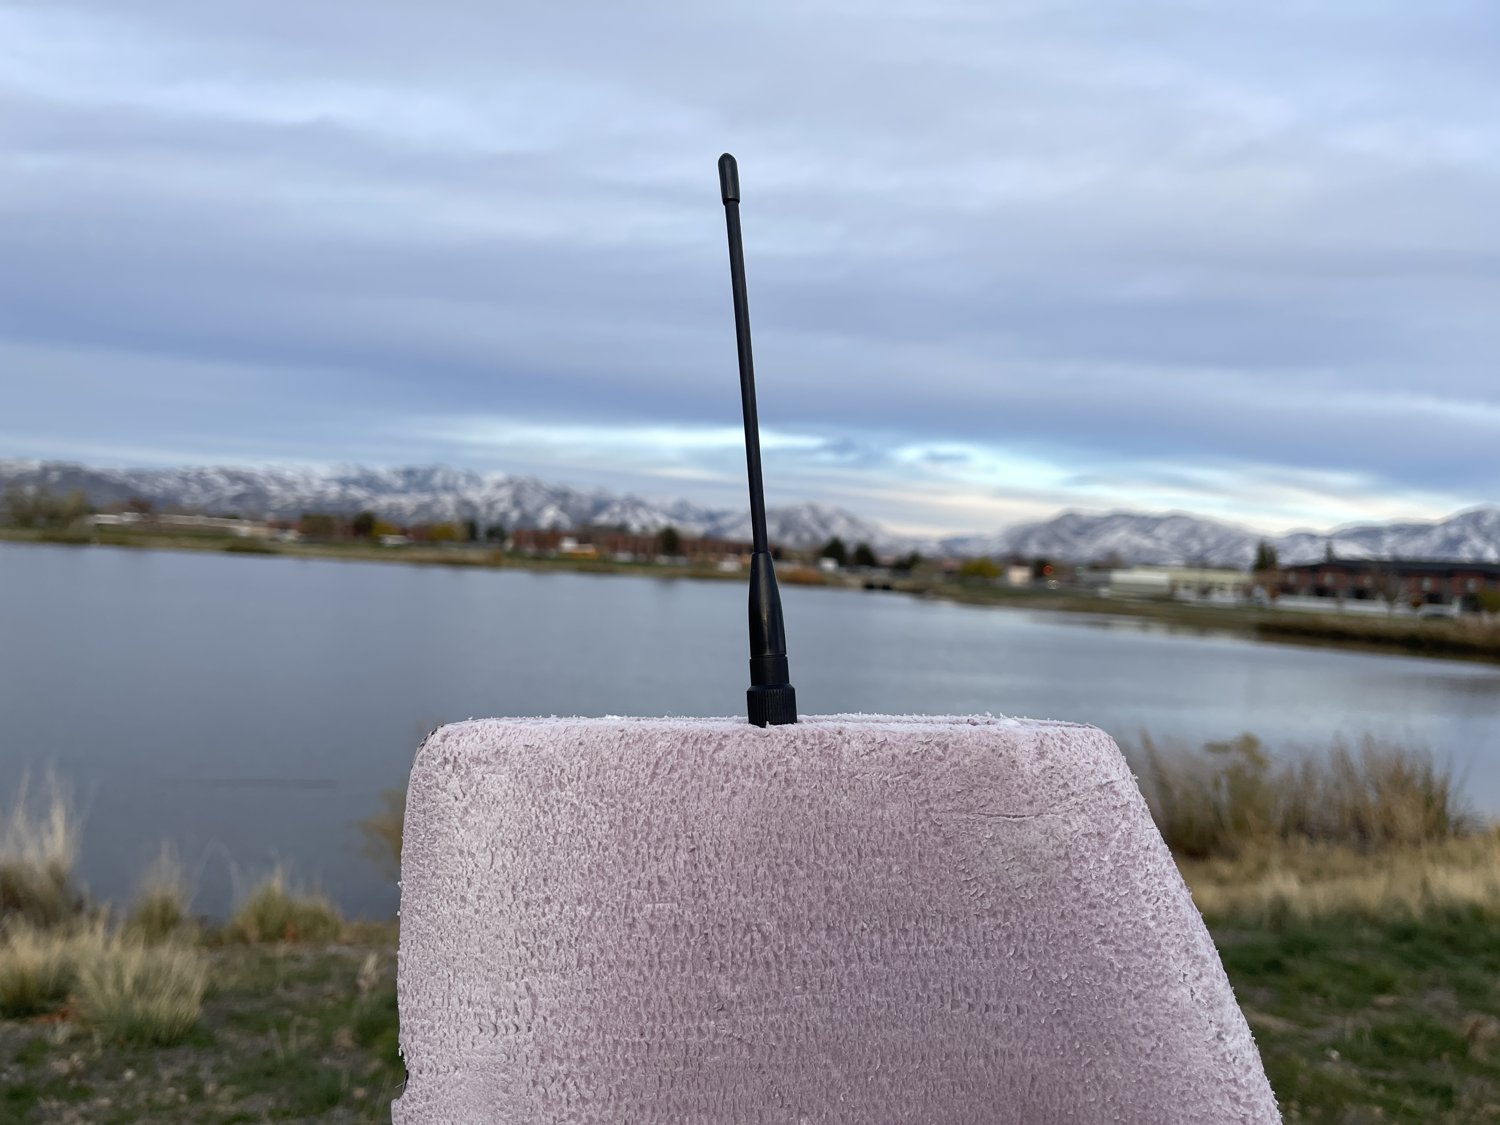
\includegraphics[height=2.55cm]{masthead_antenna}}
\caption{Wingsail hardware. (a) Printed counterweight on the forward boom
extension. (b) Tail servo in its printed bracket at the end of the lower
carbon boom, driving the tail's lower pivot. (c) Upper tail pivot bearing.
(d) Mast tube in the flanged ball-bearing unit, with the printed collar and
guard ring that form the $\pm\SI{90}{\degree}$ stops. (e) \SI{10}{dBi} LoRa
antenna at the masthead.}
\label{fig:sail}
\end{figure*}

The sail angle relative to the hull is measured below deck by an AS5600
12-bit magnetic rotary encoder at the mast step (Fig.~\ref{fig:deck}(b)). The
firmware treats one encoder revolution (4096 counts) as one revolution of the
wing, a resolution of \SI{0.088}{\degree}; the spur gearing between the mast
and the encoder is 1:1. Combined with the wind vane, this measurement closes the sail
control loop described in Section~\ref{sec:sw}.

\subsection{Integration and Balance}
\label{sec:integration}
The keel, rudder, and wing each join the hull at a single interface: the keel
bracket bolts through the reinforced keel boss, the rudder shaft turns in its
two-part bearing clamp at the transom, and the mast seats in the mast step
(Fig.~\ref{fig:cad}(b)). Each can be removed for repair without disturbing
the others. The two ballast canisters are the main trim adjustment; loading
them unevenly moves the center of mass fore and aft without changing the
hull.

The simulator's hydrostatic model (Section~\ref{sec:test}) floats a voxel
model of the CAD at its \SI{4.9}{\kilo\gram} mass. It predicts
\SI{141}{\milli\meter} of freeboard, \SI{1}{\degree} of bow-up trim, and a
total draft of \SI{307}{\milli\meter}. The righting moment stays positive to
\SI{175}{\degree} of heel, peaking at about \SI{12}{\newton\meter} near
\SI{80}{\degree}, so the ballasted keel alone makes the boat effectively
self-righting. The field test agrees: the median heel was \SI{13}{\degree},
and the boat recovered from a peak of \SI{60}{\degree} without capsizing.

At the self-trimming equilibrium the aerodynamic moment about the mast is
zero, so the sail force acts through the mast step,
\SI{107}{\milli\meter} forward of the hull's midpoint. The geometric CLR of
the hull and keel lies \SI{14}{\milli\meter} aft of the midpoint, so the COE
leads it by about \SI{120}{\milli\meter}. Because the keel's lift acts near
its quarter chord and heel adds weather helm, the effective balance is closer
than this estimate. The helm has not been measured directly; in the field
test, the heading PID held 2 to \SI{6}{\degree} of rudder to the same side on
both tacks, which suggests a small rudder-centering offset.
